% format the chapter/section details
\chapter{Results}
\label{chap:results}

% insert your text below the line
%-------------------------------------------

% contained in this file are examples for inserting figures, tables, and equations

% figure example 
\begin{figure}[h!]
    \centering % center the graphic in the text
    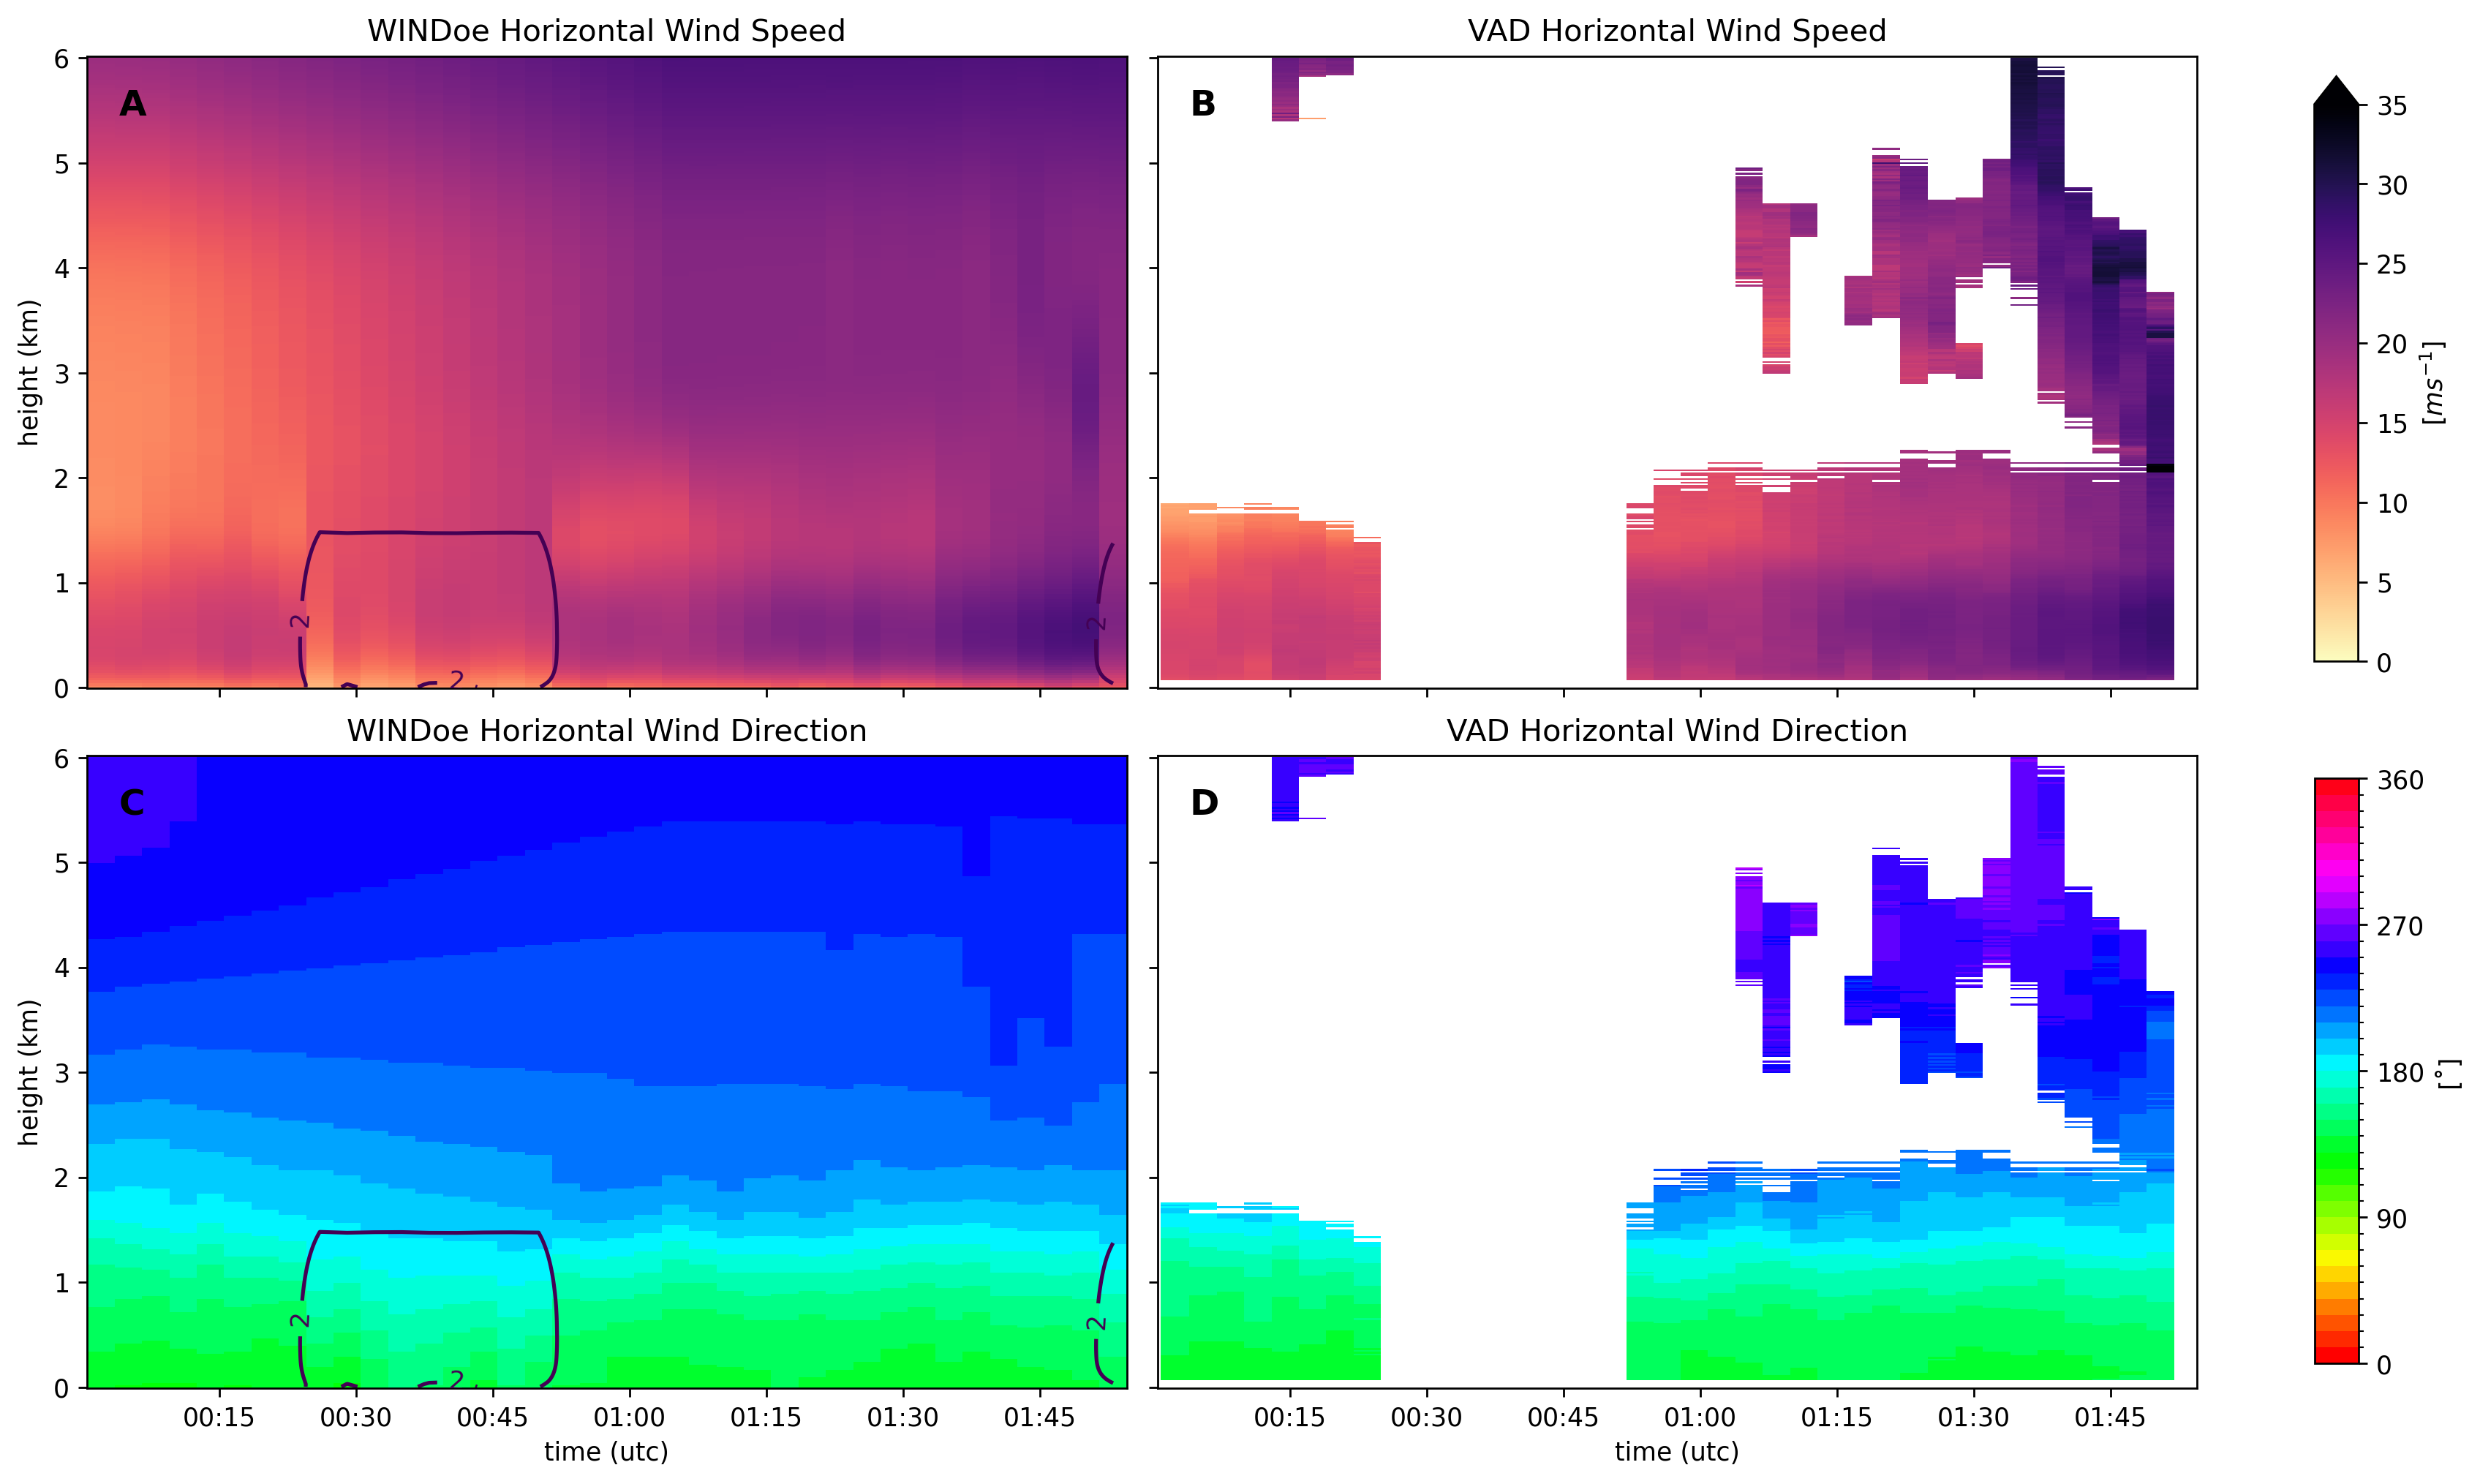
\includegraphics[width=0.7\textwidth]{figures/example.png} % include the figure
    \caption{some caption} % add a caption
    \label{fig:some_fig} % label the figure for referencing in the paper
\end{figure}

% equation example 
\begin{equation}
    \omega_h = (\frac{dw}{dy} - \frac{dv}{dz}, \frac{du}{dz} - \frac{dw}{dx}) % add equation
    \label{eq:some_eq} % label equation for referencing in paper
\end{equation}

% table example
\begin{table}[h!]
    \centering % center the table in the text
    \begin{tabular}{c|c|c} % begin the table with the text orientation of the text in table cells
        \textbf{variable} & \textbf{variable 2} & \textbf{variable 3} \\\hline % headers
        test & test & test\\ % values (this is one row)
        test & test & test\\ % values (this is one row)
        test & test & test\\ % values (this is one row)
    \end{tabular}
    \caption{some caption} % add a caption
    \label{tab:some_table} % label table for referencing in paper
\end{table}